\documentclass[12pt]{article}
\usepackage{geometry}                % See geometry.pdf to learn the layout options. There are lots.
\geometry{a4paper}                   % ... or a4paper or a5paper or ... 
%\geometry{landscape}                % Activate for for rotated page geometry
%\usepackage[parfill]{parskip}    % Activate to begin paragraphs with an empty line rather than an indent
\usepackage{graphicx}
\usepackage{amssymb}
\usepackage{epstopdf}
\usepackage{pdfpages}
\usepackage{hyperref}
\DeclareGraphicsRule{.tif}{png}{.png}{`convert #1 `dirname #1`/`basename #1 .tif`.png}

\title{Cognitive influences in language evolution: Supporting Materials}
\author{Padraic Monaghan \& Se\'{a}n Roberts}
%\date{}                                           % Activate to display a given date or no date

\begin{document}
\maketitle
%\section{}
%\subsection{}

\tableofcontents

\section{Introduction}

These are the supporting materials for Monaghan \& Roberts (2018). All data and scripts are available in a github repository: 

\hyperref[https://github.com/seannyD/BorrowingFreqAoA]{https://github.com/seannyD/BorrowingFreqAoA} .

\newpage
\section{English data (study 1)}

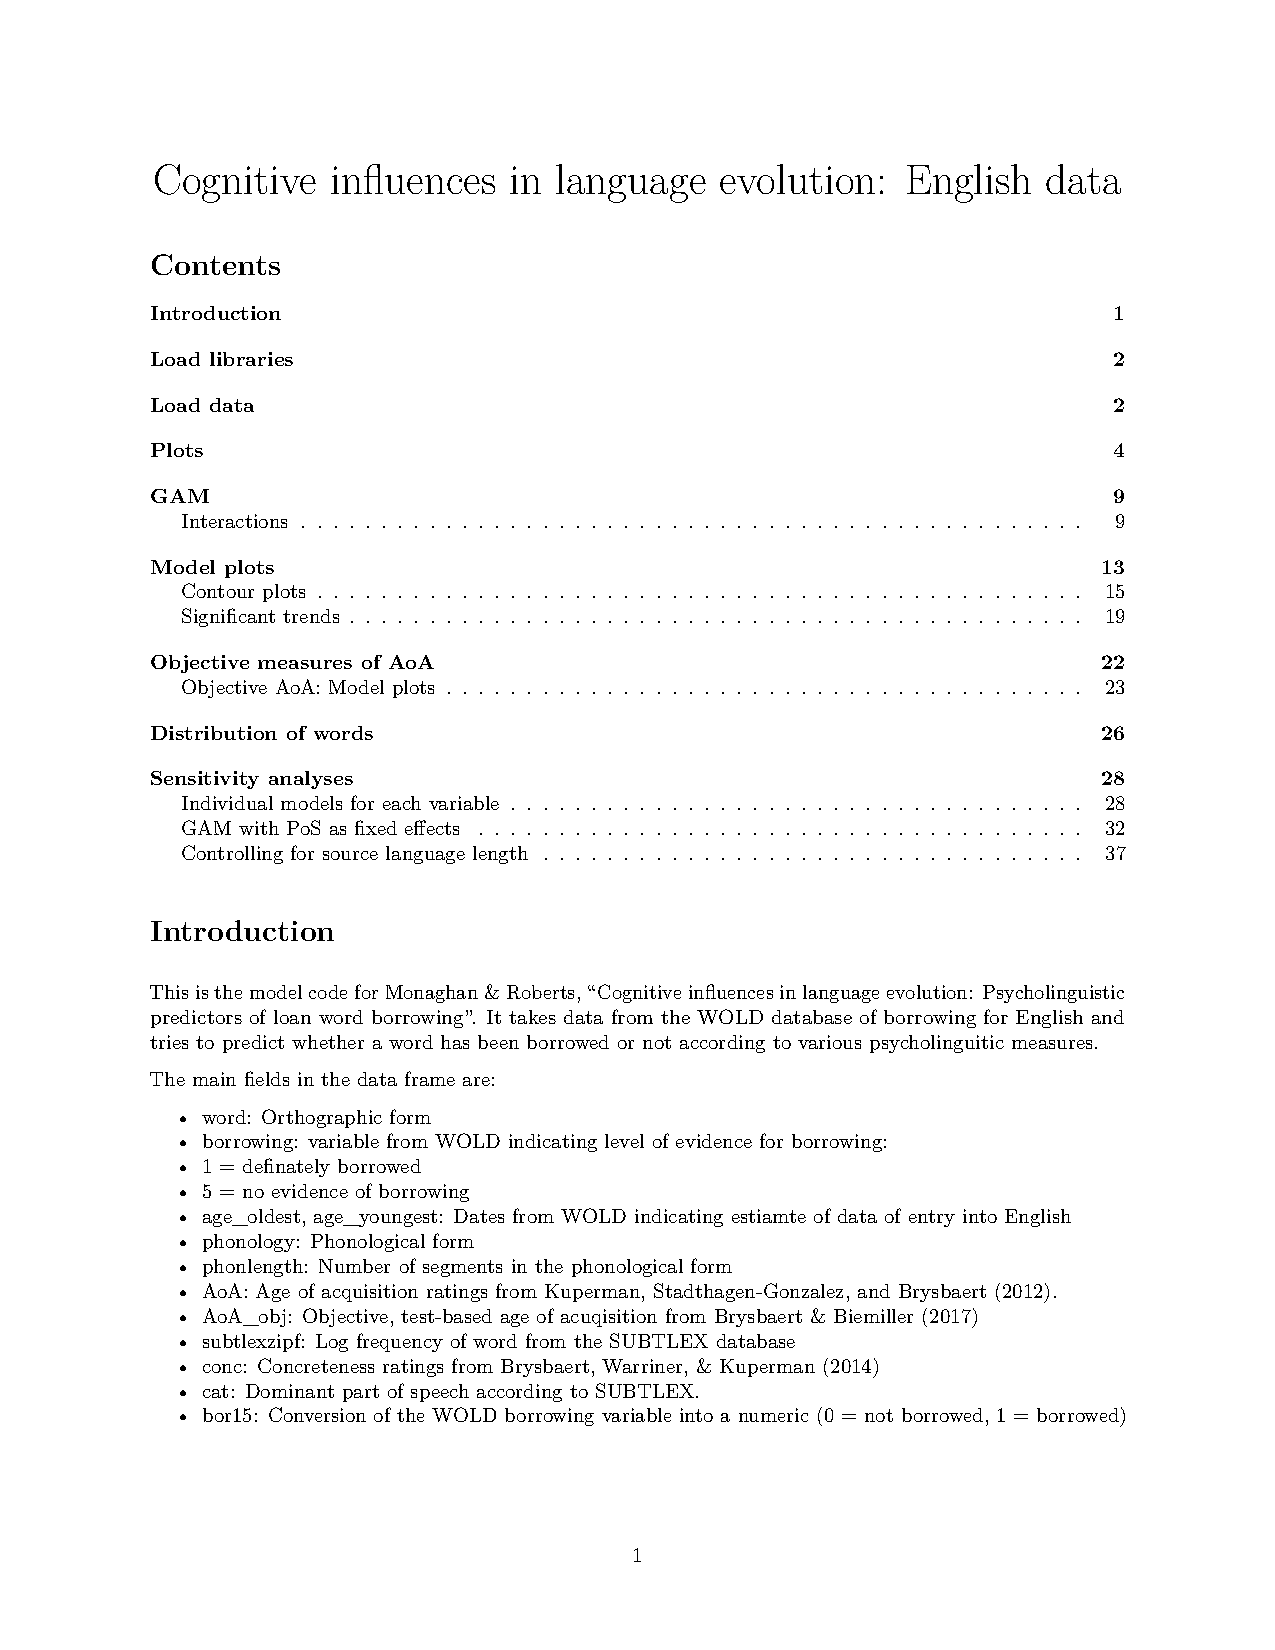
\includepdf[pages=-]{../analysis/loanwords_gam.pdf}
\newpage
\section{Dutch data (study 2)}

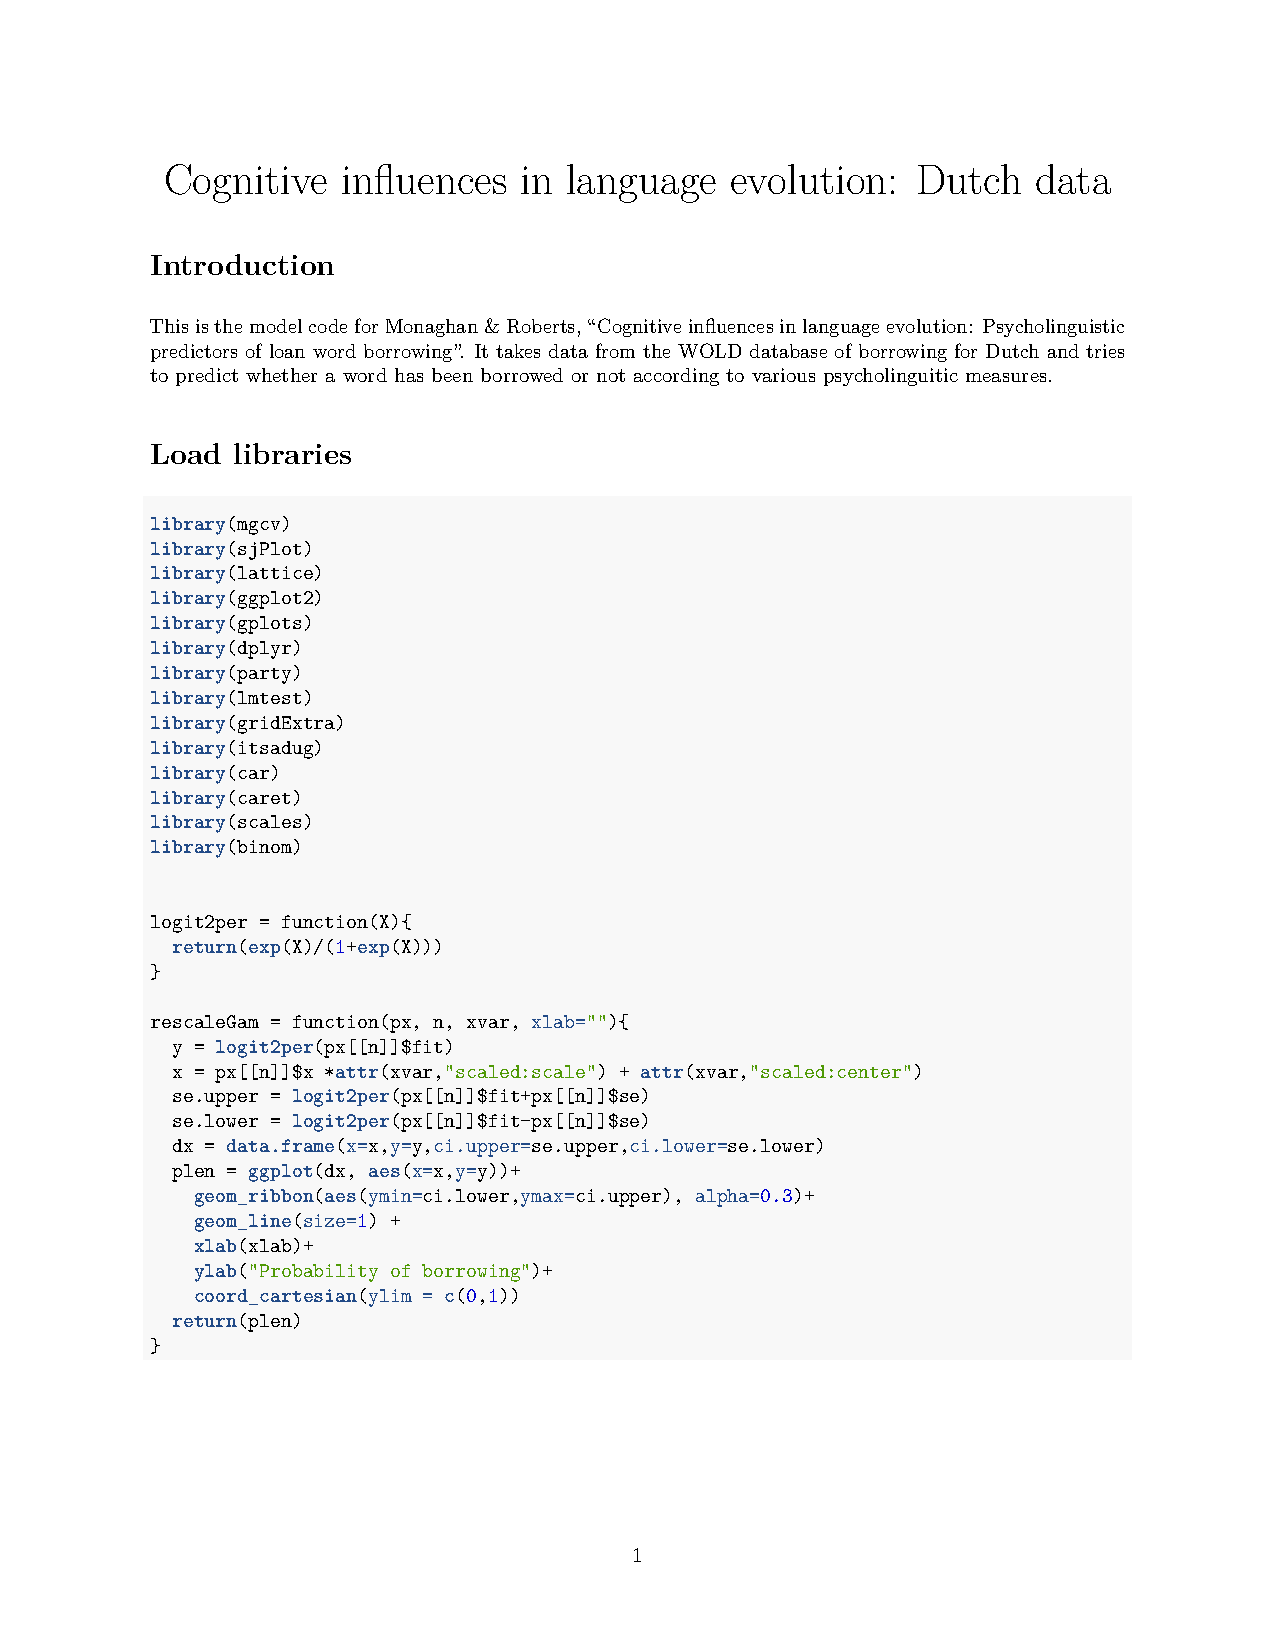
\includepdf[pages=-]{../analysis/loanwords_gam_Dutch.pdf}
\newpage
\section{Combined English and Dutch analysis}

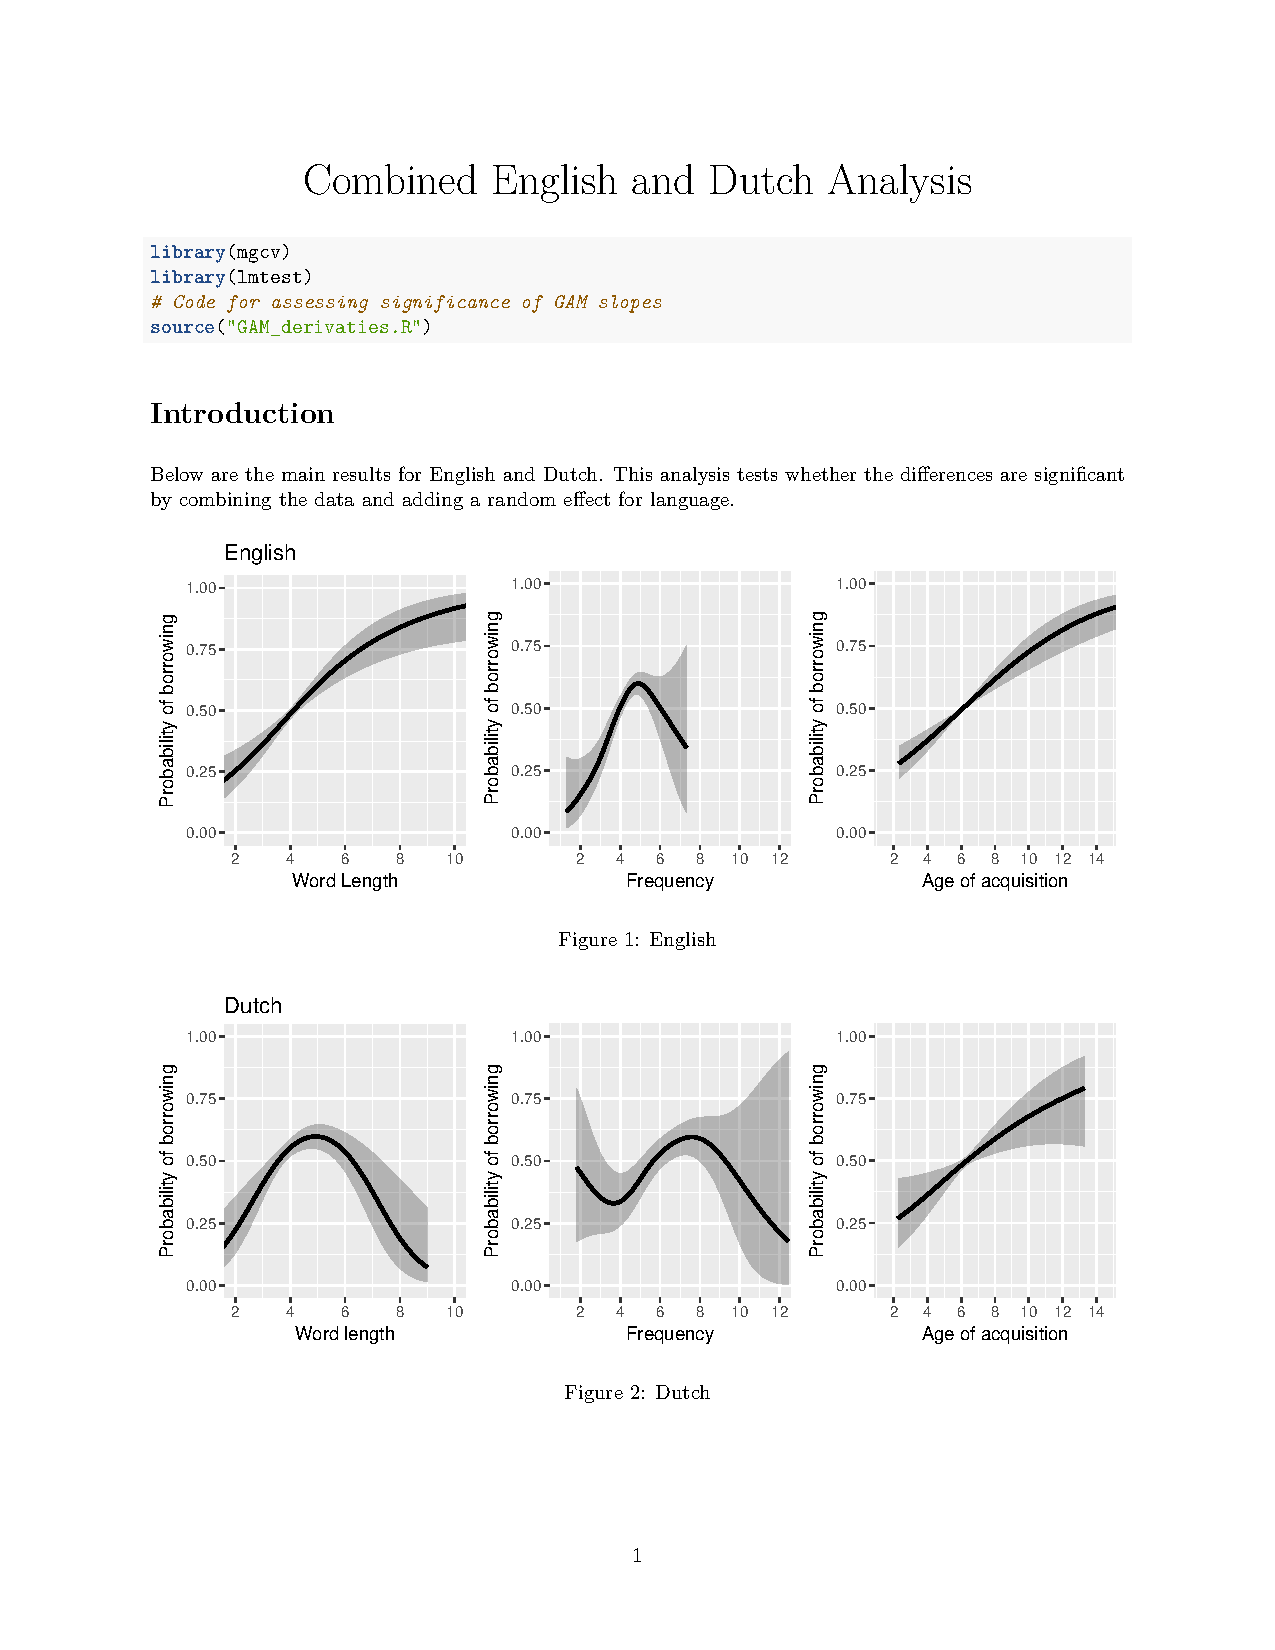
\includepdf[pages=-]{../analysis/CombinedEnglishAndDutchAnalysis.pdf}
\newpage
\section{Rates of change (study 3)}

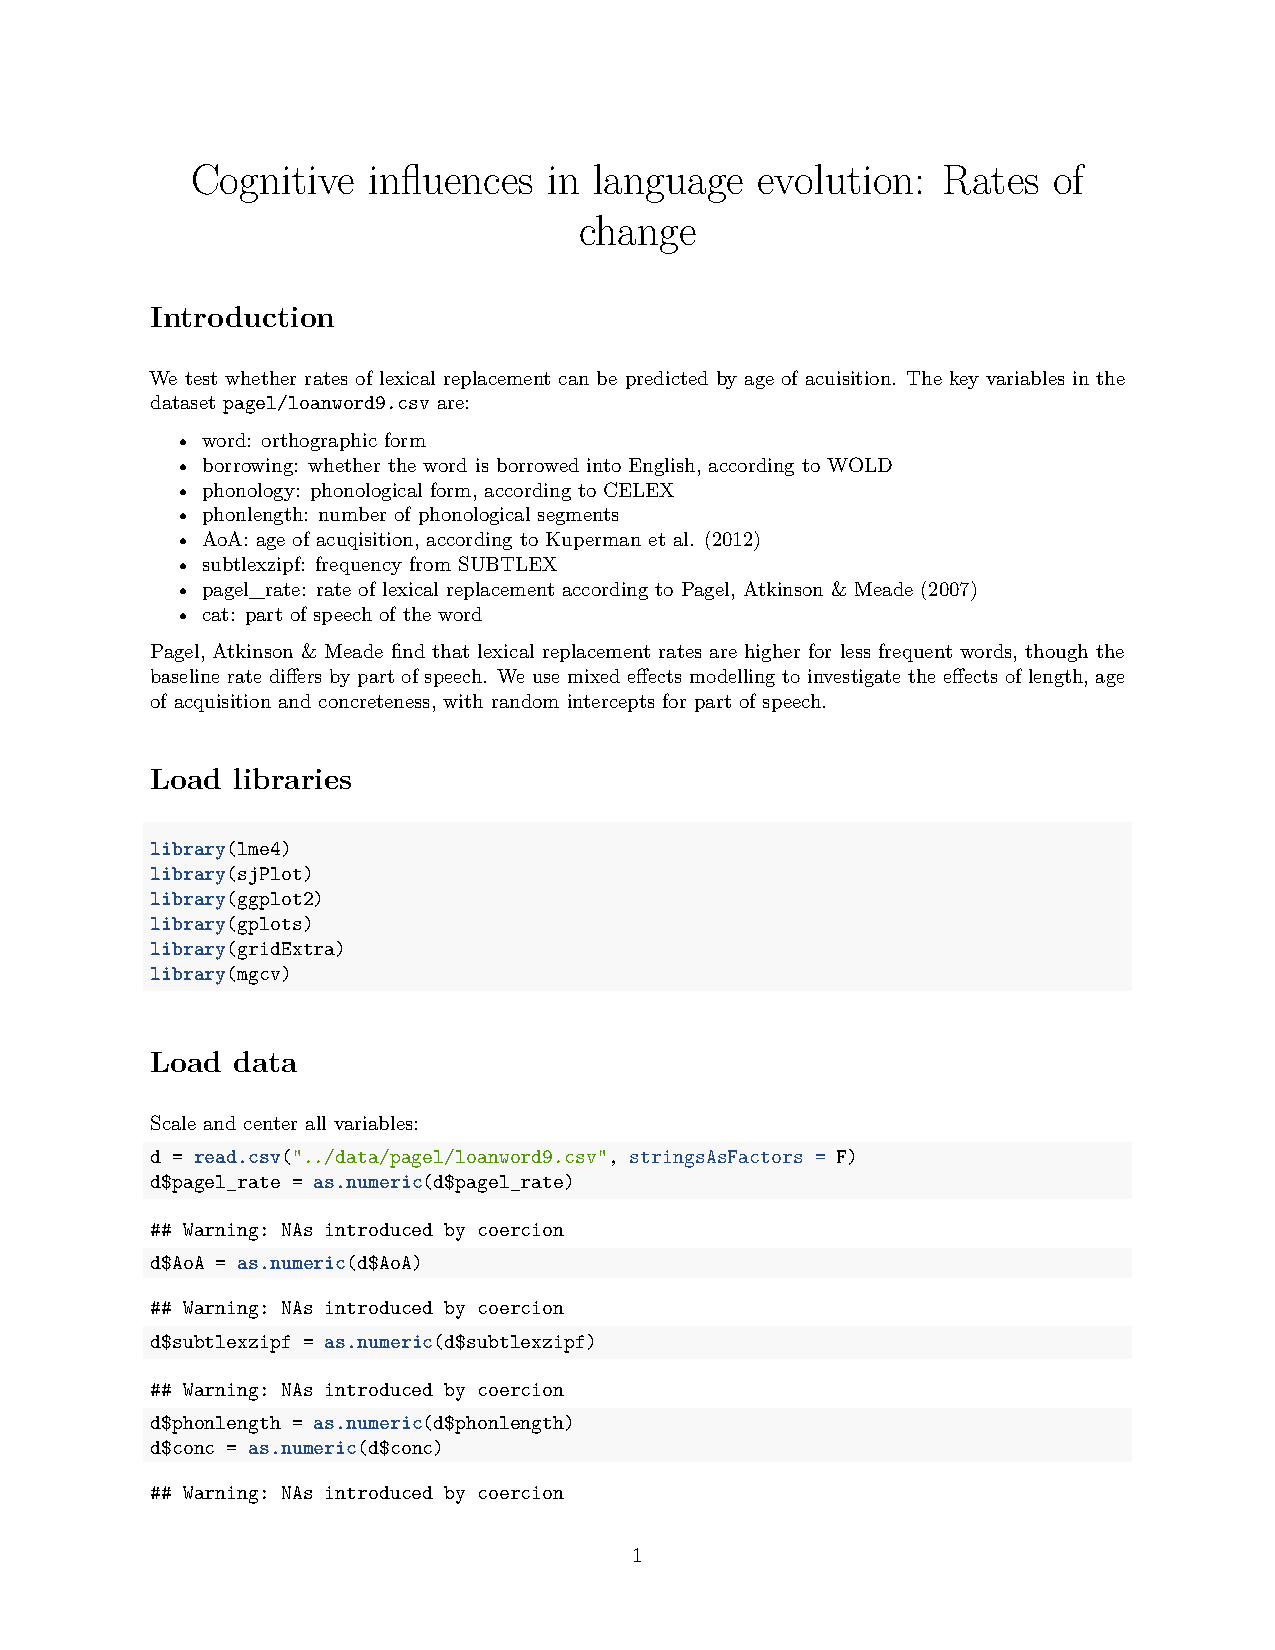
\includepdf[pages=-]{../analysis/loanwords_pagel.pdf}
\newpage
\section{Types of borrowing in Old English (study 4)}

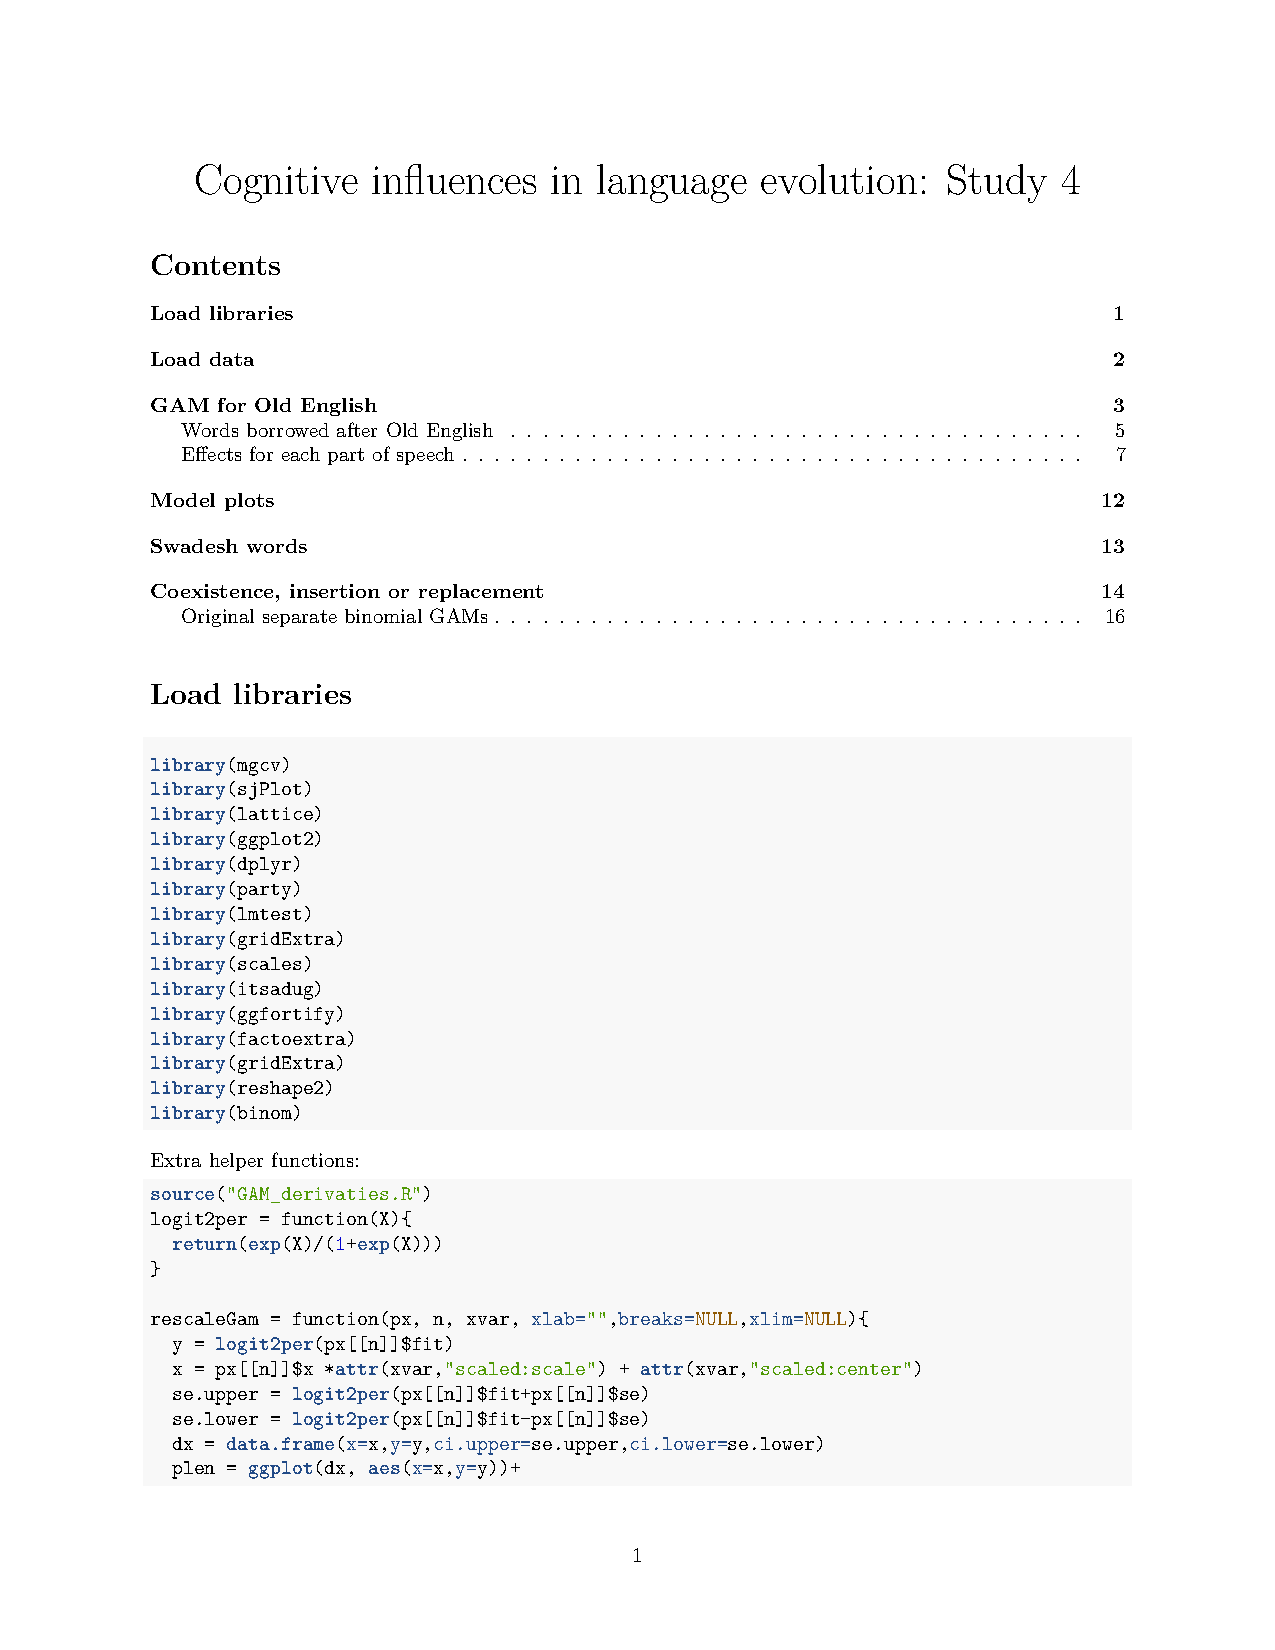
\includepdf[pages=-]{../analysis/loanwords_oldenglish_swadeshborrowing_borrowingeffect.pdf}

\end{document}  